\documentclass[12pt,letterpaper]{article}

\usepackage{listings}

\usepackage{hyperref}
\usepackage{amsmath}
\usepackage{listings}
\usepackage{graphicx}
\usepackage{textcomp}
\usepackage{subfig}

\begin{document}
\title{Evac Sim: Fall 2020 CSS600 }

\author{Justin Downes and Chris Smith}
\date{December 2020}
\maketitle

\begin{abstract}
Simulating large scale evacuation is cost-prohibitive in terms of realism and
required man-hours. Agent-based simulation supports laying out a floor plan,
modeling behaviors and at least capturing some flavor of how a real evacuation
might play out. This research uses NetLogo to vary floor plans and capture the
average escape times for the agents, focusing on the difference between two
speeds of agents, slow and medium, as  the number of people was increased.
\end{abstract}
\section {Introduction}
Talk about problem background
 
\subsection{Previous Work}
The literature abounds with previous efforts in this area.
\cite{almeidaCrowdSimulationModeling2013} 
\cite{kneidl}
\cite{kuligowskil}
\cite{abmEvac}
\cite{zhouSimulationPedestrianEvacuation2019}

This paper is key as it is extremely similar and a NetLogo implementation.  We should know this paper and incorporate into our paper \cite{prioritEvac}
\subsection {Approaches}
Talk about various modeling approaches to this problem   . mainly this paper \cite{almeidaCrowdSimulationModeling2013} 
\section {Methodology}

Our main goal was to hone in on the narrow situations in which we can detect patterns given our constrained simulation environment.  Due to the constraints of the  NetLogo environment, described further below, we are force to simplify various aspects of our model.  These simplifications though, provide us the opportunity to explore where emergent properties may arise in our agent's behavior\ref{emergentBehavior}.


%The simulation itself is straightforward, and makes novel use of the Behavior Space facility, which we wrapped in a Python driver making use of pytest which is laid out in scripts/tests/test\_fire\_sim.py
\subsection{Environment}

Our simulations utilized the NetLogo modeling environment \footnote{https://ccl.northwestern.edu/netlogo/}.  NetLogo was developed to provide an easy environment to simulate multi-agent models for educators and researchers with non programming backgrounds \cite{netlogo}.  The environment is made up of patches and agents.  The patches can be thought of the properties of the world which are accessed per cell in a grid layout.  The agents are objects that can interact with the world as well as each other.  While both agents and patches can maintain their own states, only agents can move around through the world and so can change their relationship to patches.


\begin{figure}[!h]
  \centering
  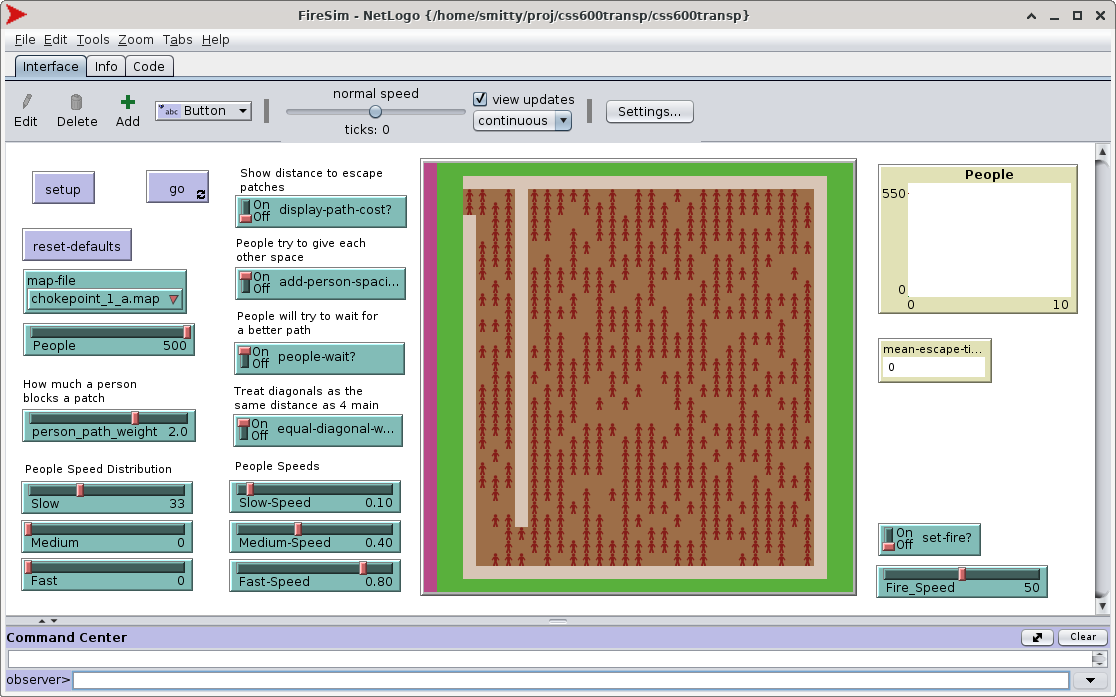
\includegraphics[width=\linewidth]{./figures/fire_sim_ui.png}
  \caption{Evac Sim UI implemented in NetLogo}
\end{figure}

One of the foundations of our simulation efforts was the ability to run experiments on a variety of maps, which mostly incrementally changed a key feature.  In order to accomplish this we implemented a custom map loader in NetLogo such that we could quickly develop custom layouts externally and procedurally load them at experiment time \ref{expEnv}.  The method of loading maps involves reading a file in line by  line which reflected a NetLogo list.  This list was then used to sequentially set the patch to the corresponding state, be it safety patch, grass, floor, or wall.  The code for loading a map and an sample of a map file are provided below.



\begin{lstlisting}[language=lisp, caption={Map loading procedure in NetLogo},captionpos=b]

to load-map
  file-open map-file
  let row  ydim
  while [not file-at-end?]
  [
    ; read each line in	
    let linestr file-read-line

    ; load line into list variable
    let line read-from-string linestr
    let col  0 - xdim

    ; for each element in list set the patch color to a value
    ; from a table of color mappings
    foreach line [
      
      [x] ->
      ask patch col row [ set pcolor table:get map_table x ]
      set col (col + 1)
    ]
  set row (row - 1)
  ]
  file-close
end
\end{lstlisting}

\begin{lstlisting}[language=lisp, caption={Example map file, 3 rows},captionpos=b]
[3 0 0 2 2 2 2 2 2 2 2 2 2 2 2 2 2 2 2 2 2 2 2 2 2 0 0]
[3 0 0 1 1 1 1 2 1 1 1 1 1 1 1 1 1 1 1 1 1 1 1 1 2 0 0]
[3 0 0 2 1 1 1 2 1 1 1 1 2 1 1 1 1 1 2 1 1 1 1 1 2 0 0]
\end{lstlisting}

Since our map creation needs were constrained to the few experiments that we planned to execute we did not implement a procedural way to generate maps.  This functionality, while one of our stretch goals, had to be dropped in the interests of deadlines.  If one were to expand upon our work then there are number of mechanisms to generate layouts \cite{mirahmadiNovelAlgorithmRealtime2012} such that further experiments could be devised without the human intensive effort of generating maps by hand.  Such possibilities include evaluations of optimal floor plans through a guided search or ablative studies on the subtle modifications of ideal floor plans.

Our simulation grid world is governed by the patch type.  The safety patch (pink) is used as the foundation for our pathing algorithm described here\ref{move}.  The grass and floor patches (green and brown) are areas in which agents can  move freely.  The two different types of patches are not just for aesthetics but are a residual from original plans to implement a fire aspect which would have burnt differently on different patches.  The final patch type is the wall (light brown) which blocks agents from moving through.

The agent's themselves are also defined fairly simply.  They have the speed at which they move, a value greater than 0 and less than 1.  They also have an internal counter for how long they have been on the map which is used to calculate the mean escape time.  This value increments on each global tick unless the agent has reached a safety patch.  In order to allow for ease of experimentation there are 3 groups of agents labeled slow, medium, and fast.  Despite the label semantics, each group can be assigned its own speed depending on the wishes of the experimenter.  During each movement step the agent moves the speed of the group that they are assigned to.  The experimenter can also set the number of agents in the environment from 0 to 500 before each simulation as expressed by the parameter $P$ below.  A helper function that we provide is the ability to maintain the ratio of numbers of slow, medium, and fast agents no matter the total number of agents.  This ratio is calculated in the following algorithm where $S$, $M$, and $F$ are the values specified by the experimenter in sliding values between 0 and 10.

\begin{equation}
\text{count of slow people} =\frac { S} {S + M + F} * P
\end{equation}

\subsection{Movement Mechanisms} \label{move}
In this section we will go over the mechanisms which dictate how our agents move throughout the environment.  Traditionally, in an environment where an agent is moving towards a goal, each agent's path to that goal will be calculated individually through the environment\footnote{http://www.cs.us.es/~fsancho/?e=131}.  In our situation we implemented a simplified pathing algorithm which instead calculates global weights for each environmental patch in which all agents flow to the lowest weight.  These weights grow in relation to their distance to the safety patches and as agents move over them by imparting their own weight to the patch.  This simplified pathing allows for much quicker computation of routes and therefor quicker executions of simulations for our experiments.

The following will provide an overview of how the weighting mechanisms work and the choices agents make on whether to move.  The foundation of movement is the weight of a given patch, or the cost as described below. The cost metric is defined as the distance from the patch to be considered $P$ and the nearest safety patch $P_s$.  While there may be many safety patches, for the sake of brevity, we assume that $P_s$ is resolved \emph{a priori} as the closest.  We can confidently declare this since the weighting implementation iteratively grows from each safety patch such that when it reaches a candidate patch it has been reached by the closest one.  This distance cost is also modified by the presence of an agent, $Agent(P)$, on that patch.  This agent's weight, $A_w$, is configurable by the user.  Of important note is that the weight is calculated independently of agents that may reside on patches between a patch and the safety patch.  This is the simplified pathing mechanism at work in that only local environment calculations are conducted.
\begin{align}
cost(P)  = distance(P_s, P) + Agent(P) * A_w \nonumber \\
Agent(P)=
\begin{cases}
1, & \text{Agent Present}  \\
0, & \text{Agent Not Present} 
\end{cases}
\end{align}

The distance measurement is not as simple as calculating the Euclidean distance.  Since our environment is a grid world that is inhabited by blocking obstacles we can only consider movement in either the 4 cardinal directions or the 8 neighboring directions.  These two options, which are additionally configurable by the user, determine how the distance between patches are measured.  The distance between 2 points $P_1$ \& $P_2$ is optionally defined by the flag $equal-diagonal-weight?$.  If false the distance is the Manhattan distance \footnote{ https://www.sciencedirect.com/topics/mathematics/manhattan-distance}. If true the distance is the Chebyshev distance \footnote{https://en.wikipedia.org/wiki/Chebyshev\_distance}. While this algorithm for distance works in an open world it doesn't account for the blocking obstacles.  This is another side effect of how the actual implementation works.  By growing outward from the safety patches and around obstacles the actual distance calculation is only ever considered for patches that are next to each other.  This makes our implementation a narrow case of the algorithm below in that all distances we calculate equal 1 and the real choice is how we choose the next patches as either the Manhattan or the Chebyshev neighborhood.
\begin{align}
distance(P_1, P_2)  = \nonumber\\
equal-diagonal-weight?=
\begin{cases}
	max(|x_1-x_2|, |y_1-y_2|), & True \\
	|x_1-x_2|+ |y_1-y_2|, & False
\end{cases}
\end{align}

Now that we have our patch weights to inform our movement decisions it is time to actually make the decision of where to move to.  For this choice we simply choose the neighbor patch that has the lowest cost, where the neighbors are defined as the 4 patches above, below, right, and left of our current patch.  Once we know which patch is lowest we take the vector at that patch and multiply it by our agent's speed.  So, for a given agent $A$ the vector to move is given by the vector of the lowest cost neighbor patch times our agent's speed. 


\begin{equation}
move(A) = V( min(cost(neighbors_4 (A_p))) ) * S_a
\end{equation}

\begin{align}
neighbors_4 (P)  = \{patch(P_x - 1, P_y -1), patch(P_x + 1, P_y -1), \nonumber \\ 
patch(P_x - 1, P_y + 1),patch(P_x + 1, P_y + 1)\}   
\end{align}


We have an additional parameter to account for situations where the cost of all neighboring patches is greater than the current patch. The flag $people-wait?$ allows simulators to decide whether or not to stay put and wait for a better patch or to always move even if the new patch has a higher cost.  This flag redefines the $move(A)$ function as $move(A)$ if the flag is false and if the cost of the current patch is less than $move(A)$ then to not move.
\begin{equation}
people-wait?=
\begin{cases}
min(cost(A_p), move(A)), & True \\
move(A), & False
\end{cases}
\end{equation}

Another phenomena we wished to capture is the ability for agent's to give each other space.  This is configurable through the $add-person-spacing?$ flag.  When the flag is true the cost of a patch is redefined to be the normal cost plus the sum of all the neighbors with agents times the agent's weight divided by 10.  This scaling factor of $1/10$ has been determined through trial and error and is something that could be exposed to user control in the future.  For ease of implementation and increased computation time the actual calculation is done from the perspective of the agent in that each agent has their scaled weight applied to its patch neighbors.

\begin{align}
add-person-spacing?= \nonumber  \\
\begin{cases}
	cost(P) + \sum Agent(neighbors_4(P)) * A_w / 10, & True \\
	cost(P), & False
\end{cases}
\end{align}

The grid world, while maybe too much of a simplification of real world dynamics, enables us to implement complex behaviors through simple straightforward algorithms.  These complex behaviors have enabled us to conduct a few interesting experiments described in the following sections.

\section{Experiments}

This should be about the underlying approach to devising and goals of our experiments

\subsection{Experimental Environment} \label{expEnv}
This section describes our experiment harness that we built using NetLogo's
Behavior Space functionality.

Behavior Space supports supplying simulation arguments via an XML document,
invoking the NetLogo engine via a script pointing to the XML, and then capturing
the results via the standard output.

This lends itself to scripting via Python \footnote{https://www.python.org/}. The goal had been to extract the
initial Behavior Space XML content directly from the .nlogo file, and then craft
a SQLAlchemy \footnote{https://www.sqlalchemy.org/} model on the fly that would support storing results in an RDBMS,
e.g. SQLite \footnote{https://sqlite.org/index.html}. That proved out of reach due to the advanced nature of SQLAlchemy,
so a hand-crafted model was used, which makes alterations to the underlying
model more maintenance intensive.

While we stored the results in a local SQLAlchemy file, a mere update to the
connection string would allow storing results in an enterprise RDBMS to good
effect.

Another Open Source tool that was used extensively was PyTest \footnote{https://docs.pytest.org/en/stable/}. Billed as a
unit testing framework, PyTest supports breaking the problem down into granular
fixtures and then combing them in a Lego-like fashion that lends itself to the
problem space. For example, while Behavior Space allows stepped alteration of
numerical parameters in a model, swapping out map file names is not directly
supported. Implementing a Python function to generate the map file names and
then re-writing the XML was far more convenient than having distinct
experiments for each map.

And then Python's data science facilities are well-known \footnote{https://www.scipy.org/index.html}, supporting arbitrary
visualization pipelines.

\subsection{Experimental Parameters}
For the map files in use, there were 10 runs against the map files, capturing
mean-escape-time for the agents.

\begin{tabular}{ l | l }
VARIABLE & MEANING / VALUE \\
map-file & Name of map file to set up. \\
People & Number  of people. Held constant at 500. \\
person\_path\_weight & Agent blockage factor for patch \\
Slow & Percentage moving at this rate, which we set to 100 \\
Medium & Set to 0 \\
Fast & Set to 0 \\
Slow-Speed & 0.3 patches \\
Medium-Speed & 0.75 patches \\
Fast-Speed & 1.0 patches \\
add-person-spacing? & true \\
equal-diagonal-weight? & true \\
display-path-cost? & false \\
people-wait? & true \\
set-fire? & false \\
Fire\_Speed & 50 \\
mean-escape-time & output \\
\end{tabular}

\subsection{Experiments Based on Layouts}
This section will describe the different layout based experiments.  How we set them up to narrow parameters to just measure the layouts impact

\subsubsection{Chokepoint Experiment}

\begin{figure*}[ht]
  \centering
  \begin{minipage}[b]{\linewidth}
    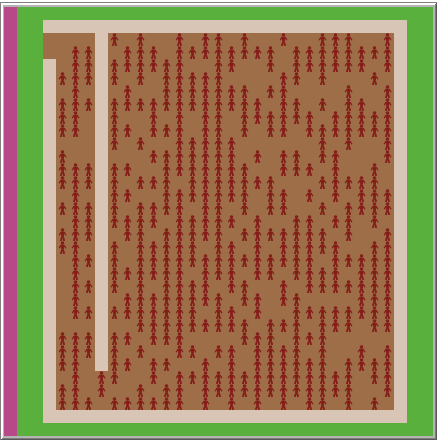
\includegraphics[width=0.15\textwidth]{./figures/chokepoint_1_a.png}
    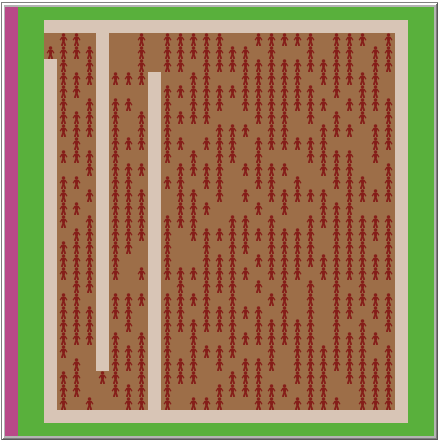
\includegraphics[width=0.15\textwidth]{./figures/chokepoint_1_b.png}
    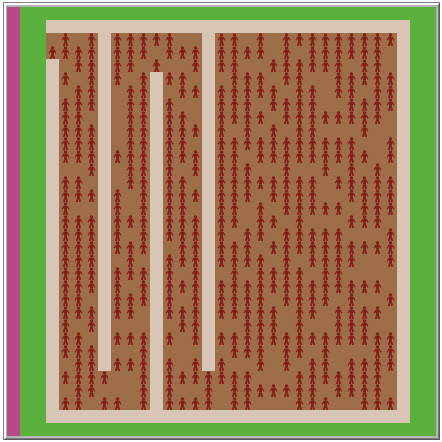
\includegraphics[width=0.15\textwidth]{./figures/chokepoint_1_c.png}
    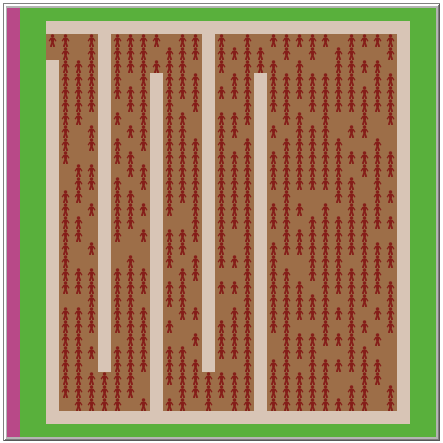
\includegraphics[width=0.15\textwidth]{./figures/chokepoint_1_d.png}
    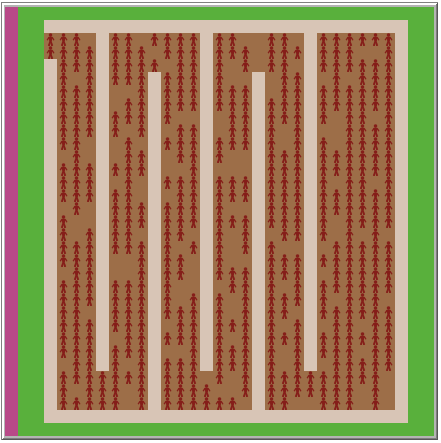
\includegraphics[width=0.15\textwidth]{./figures/chokepoint_1_e.png}
    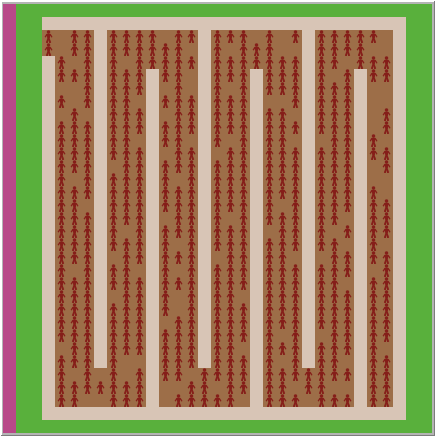
\includegraphics[width=0.15\textwidth]{./figures/chokepoint_1_f.png}
  \end{minipage}
  \begin{minipage}[b]{\linewidth}
    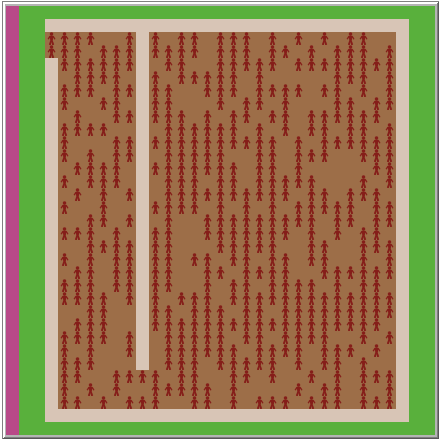
\includegraphics[width=0.15\textwidth]{./figures/chokepoint_2_a.png}
    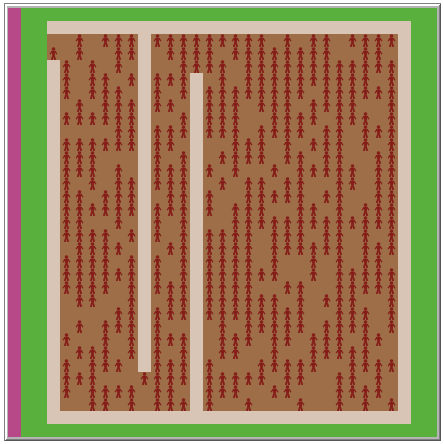
\includegraphics[width=0.15\textwidth]{./figures/chokepoint_2_b.png}
    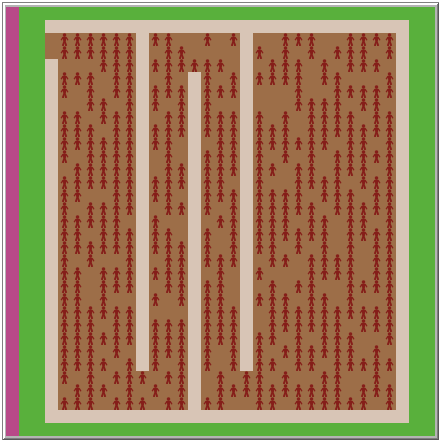
\includegraphics[width=0.15\textwidth]{./figures/chokepoint_2_c.png}
    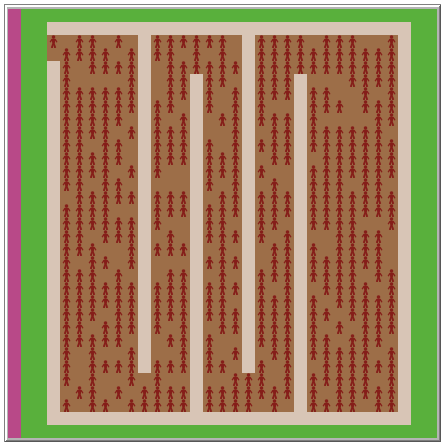
\includegraphics[width=0.15\textwidth]{./figures/chokepoint_2_d.png}
    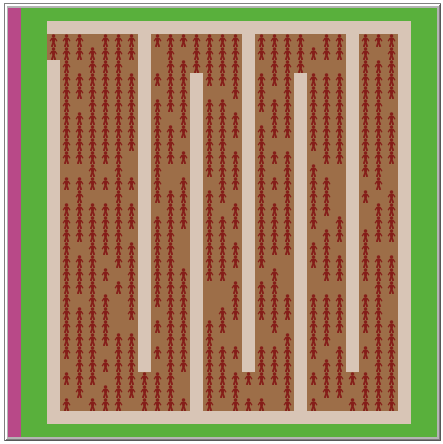
\includegraphics[width=0.15\textwidth]{./figures/chokepoint_2_e.png}
  \end{minipage}
  \begin{minipage}[b]{\linewidth}
    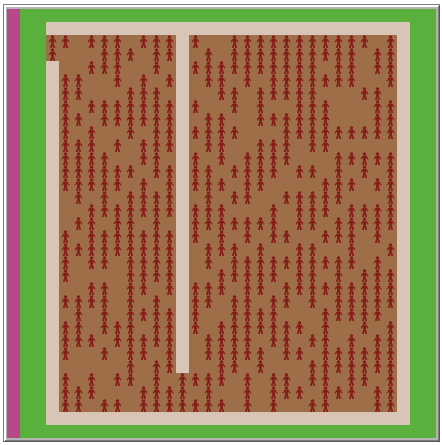
\includegraphics[width=0.15\textwidth]{./figures/chokepoint_3_a.png}
    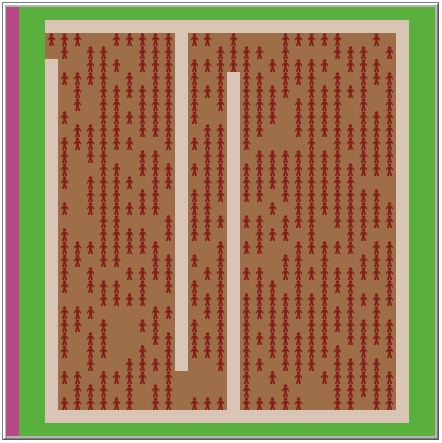
\includegraphics[width=0.15\textwidth]{./figures/chokepoint_3_b.png}
    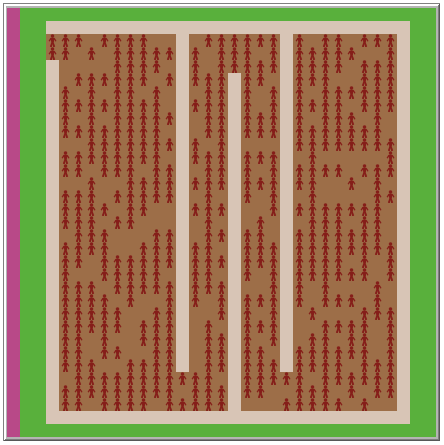
\includegraphics[width=0.15\textwidth]{./figures/chokepoint_3_c.png}
    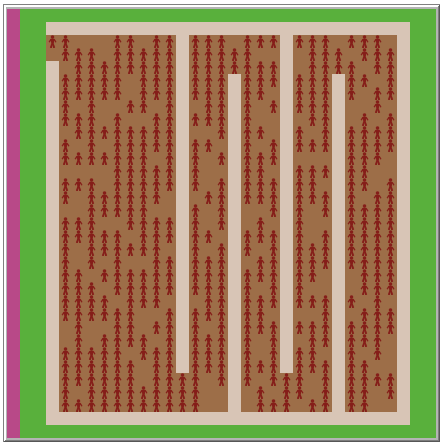
\includegraphics[width=0.15\textwidth]{./figures/chokepoint_3_d.png}
  \end{minipage}
  \caption{Chokepoint Maps}
\end{figure*}

\subsubsection{Exit Dimensions}

\begin{figure*}[ht]
  \centering
  \begin{minipage}[b]{.75\linewidth}
    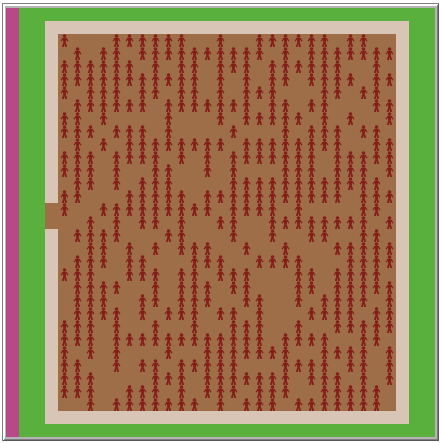
\includegraphics[width=0.3\textwidth]{./figures/exit_dims_2_a.png}
    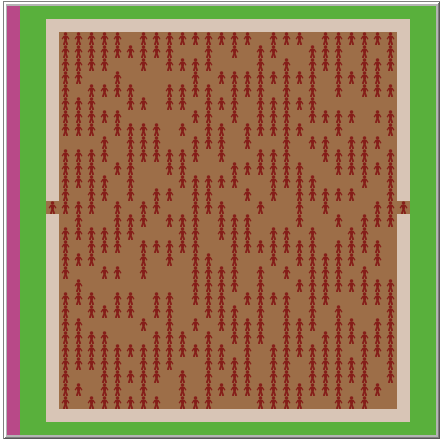
\includegraphics[width=0.3\textwidth]{./figures/exit_dims_2_b.png}
    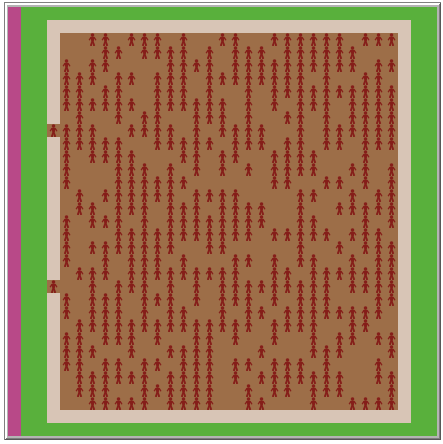
\includegraphics[width=0.3\textwidth]{./figures/exit_dims_2_c.png}
  \end{minipage}
  \begin{minipage}[b]{.75\linewidth}
    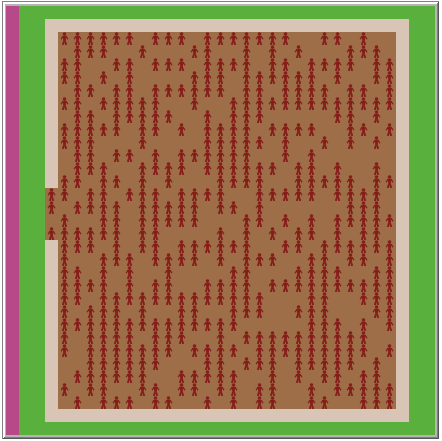
\includegraphics[width=0.3\textwidth]{./figures/exit_dims_4_a.png}
    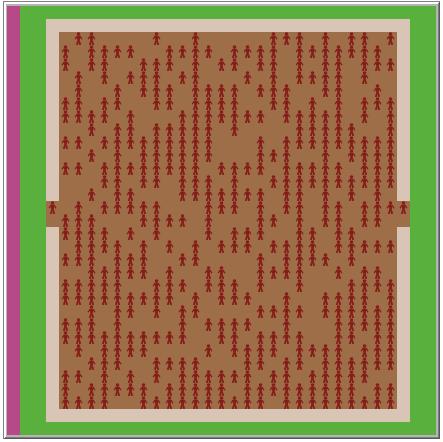
\includegraphics[width=0.3\textwidth]{./figures/exit_dims_4_b.png}
    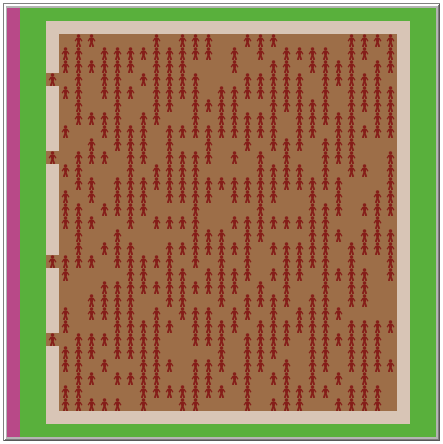
\includegraphics[width=0.3\textwidth]{./figures/exit_dims_4_c.png}
  \end{minipage}
  \begin{minipage}[b]{.75\linewidth}
    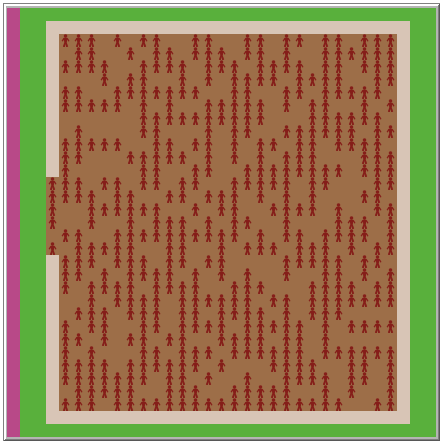
\includegraphics[width=0.3\textwidth]{./figures/exit_dims_6_a.png}
    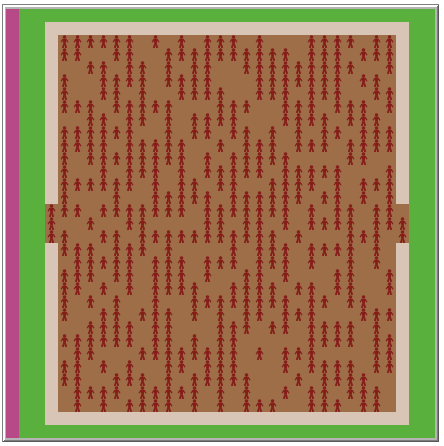
\includegraphics[width=0.3\textwidth]{./figures/exit_dims_6_b.png}
    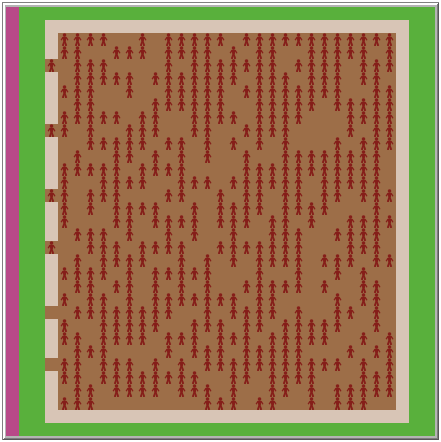
\includegraphics[width=0.3\textwidth]{./figures/exit_dims_6_c.png}
  \end{minipage}
  \begin{minipage}[b]{.75\linewidth}
    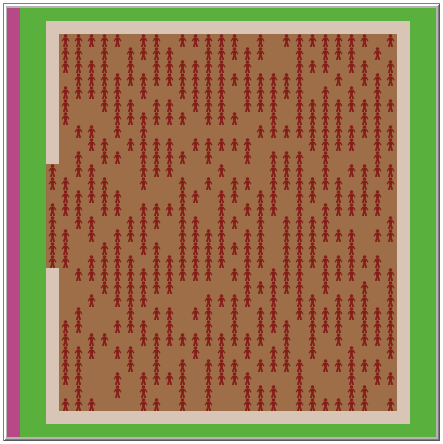
\includegraphics[width=0.3\textwidth]{./figures/exit_dims_8_a.png}
    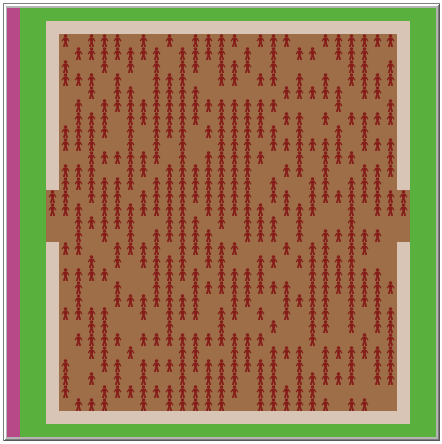
\includegraphics[width=0.3\textwidth]{./figures/exit_dims_8_b.png}
    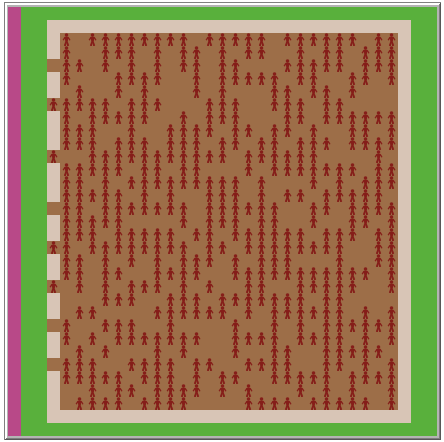
\includegraphics[width=0.3\textwidth]{./figures/exit_dims_8_c.png}
  \end{minipage}
  \caption{Exit Dimensions Maps}
\end{figure*}
\subsection{Experiments Based on Agent Features}

This section will cover our experiments based on modifying the agent's speed distributions.


\subsection{Experiments Replicating Emergent Crowd Behaviors} \label{emergentBehavior}
- mainly from this paper \cite{almeidaCrowdSimulationModeling2013}  .  This section will cover how we hope to see these emergent behaviors in our environments even though we use a simplified pathing strategy.  This could lead to simpler models with less resource requirements.



\begin{figure}[!htbp]
  \centering
  \subfloat[Evacuation with no herding ]{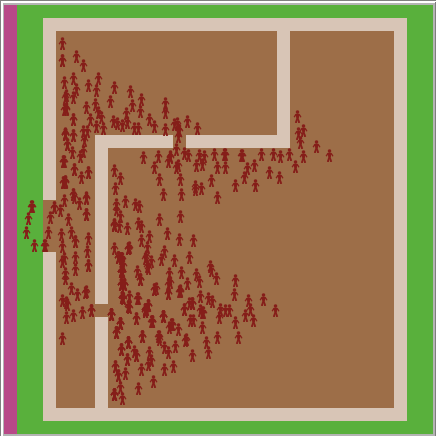
\includegraphics[width=0.4\textwidth]{./figures/Herding1.png}\label{fig:f1}}
  \hfill
  \subfloat[Evacuation with herding (i.e. ignoring viable exit)]{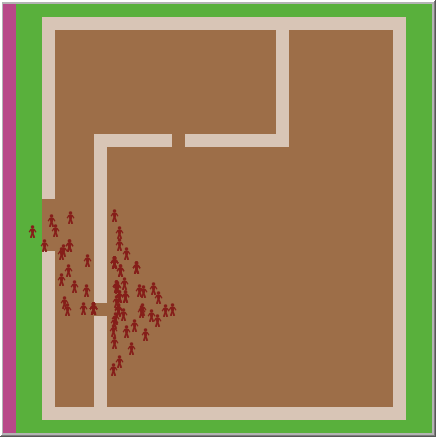
\includegraphics[width=0.4\textwidth]{./figures/Herding-2.png}\label{fig:f2}}
  \caption{Herding behavior replicated through residual escape pathing from agents that never considered the alternative route.}
\end{figure}

\begin{figure}[!htbp]
  \centering
  \subfloat[No clogging due to people not blocking paths ]{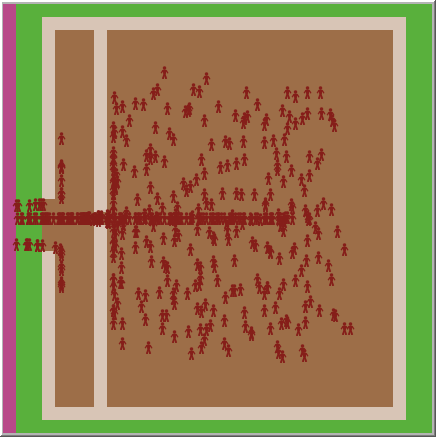
\includegraphics[width=0.4\textwidth]{./figures/clogging1_clean.png}\label{fig:f1}}
  \hfill
  \subfloat[Clogging due to increased weight per person on a patch]{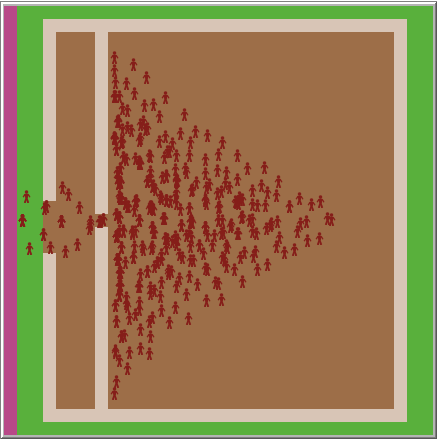
\includegraphics[width=0.4\textwidth]{./figures/clogging2_clean.png}\label{fig:f2}}
  \caption{Clogging behavior replicated through a weight attribute calculated for each patch an agent is on as well as a configurable additional weight for each agent's neighboring patch. }
\end{figure}


if we can show that we achieve similar results even though we use a simplified pathing algorithm and abm environment i think that would be insightful


%\section{Results}
%
%The results showed that adding more length to the chokepoint pipeline did not
%result in a linear increase in the exit time. Rather, the Actors resembled a
%fluid dynamics problem, reaching a uniform flow and making good their escape.
%
%More exits is better, especially if not on the same side, but there is not a
%linear increase with additional exits.
%
%
%
%need to talk about patch parameters
%\subsection{Movement Mechanisms}
%This section discusses agent and fire movement algorithms.
%
%The cost algorithm, where $P_s$ is a safety patch, where $A_w$ is the person path weight, a weight that a person adds to a patch due to blocking (this is configurable by the user)
%\begin{align}
%cost(P)  = distance(P_s, P) + Agent(P) * A_w \nonumber \\
%Agent(P)=
%\begin{cases}
%1, & \text{Agent Present}  \\
%0, & \text{Agent Not Present} 
%\end{cases}
%\end{align}
%
%This can be configured through equal diagonal weight flag. if False the Distance is the Manhattan distance \footnote{ https://www.sciencedirect.com/topics/mathematics/manhattan-distance}. If true the distance is the Chebyshev Distance \footnote{https://en.wikipedia.org/wiki/Chebyshev\_distance}
%\begin{align}
%distance(P_1, P_2)  = \nonumber\\
%equal-diagonal-weight?=
%\begin{cases}
%	max(|x_1-x_2|, |y_1-y_2|), & True \\
%	|x_1-x_2|+ |y_1-y_2|, & False
%\end{cases}
%\end{align}
%
%
%Patch to move to algorithm, where $A_p$ is the patch for a given agent, $P_x$ \& $P_y$ are the $X$ \& $Y$ coordinates for a given patch
%\begin{align}
%neighbors_4 (P)  = \{patch(P_x - 1, P_y -1), patch(P_x + 1, P_y -1), \nonumber \\ 
%patch(P_x - 1, P_y + 1),patch(P_x + 1, P_y + 1)\}   
%\end{align}
%
%\begin{equation}
%move(A) = min(cost(neighbors_4 (A_p)))
%\end{equation}
%
%Person will wait for a better patch.  This is configurable by the user. If it is on then a person will wait for a patch that is less cost than its current
%\begin{equation}
%people-wait?=
%\begin{cases}
%min(cost(A_p), move(A)), & True\\
%move(A), & False
%\end{cases}
%\end{equation}
%
%Add person spacing algorithm, people try to avoid each other, configurable through the $add-person-spacing?$ flag and the $person\_path\_weight$, $A_w$, parameter.  here, $A_w$, is scaled by a factor of 10 since it is not the weight of being in the same square as another but of being next to another person.
%
%\begin{equation}
%add-person-spacing?=
%\begin{cases}
%	cost(P) \sum Agent(neighbors_4(P)) * A_w / 10, & True \\
%	cost(P), & False
%\end{cases}
%\end{equation}
%
%\cite{mirahmadiNovelAlgorithmRealtime2012}
%\footnote{http://www.cs.us.es/~fsancho/?e=131}
%
%\subsection{Experiments}
%
%This section describes our experiment harness that we built using NetLogo's
%Behavior Space functionality.
%
%Behavior Space supports supplying simulation arguments via an XML document,
%invoking the NetLogo engine via a script pointing to the XML, and then capturing
%the results via the standard output.
%
%This lends itself to scripting via Python \footnote{https://www.python.org/}. The goal had been to extract the
%initial Behavior Space XML content directly from the .nlogo file, and then craft
%a SQLAlchemy \footnote{https://www.sqlalchemy.org/} model on the fly that would support storing results in an RDBMS,
%e.g. SQLite \footnote{https://sqlite.org/index.html}. That proved out of reach due to the advanced nature of SQLAlchemy,
%so a hand-crafted model was used, which makes alterations to the underlying
%model more maintenance intensive.
%
%While we stored the results in a local SQLAlchemy file, a mere update to the
%connection string would allow storing results in an enterprise RDBMS to good
%effect.
%
%Another Open Source tool that was used extensively was PyTest \footnote{https://docs.pytest.org/en/stable/}. Billed as a
%unit testing framework, PyTest supports breaking the problem down into granular
%fixtures and then combing them in a Lego-like fashion that lends itself to the
%problem space. For example, while Behavior Space allows stepped alteration of
%numerical parameters in a model, swapping out map file names is not directly
%supported. Implementing a Python function to generate the map file names and
%then re-writing the XML was far more convenient than having distinct
%experiments for each map.
%
%And then Python's data science facilities are well-known \footnote{https://www.scipy.org/index.html}, supporting arbitrary
%visualization pipelines.
%
%\subsubsection{Experiments Based on Layouts}
%The length of the exit passage was increased gradually
%\begin{figure}
%  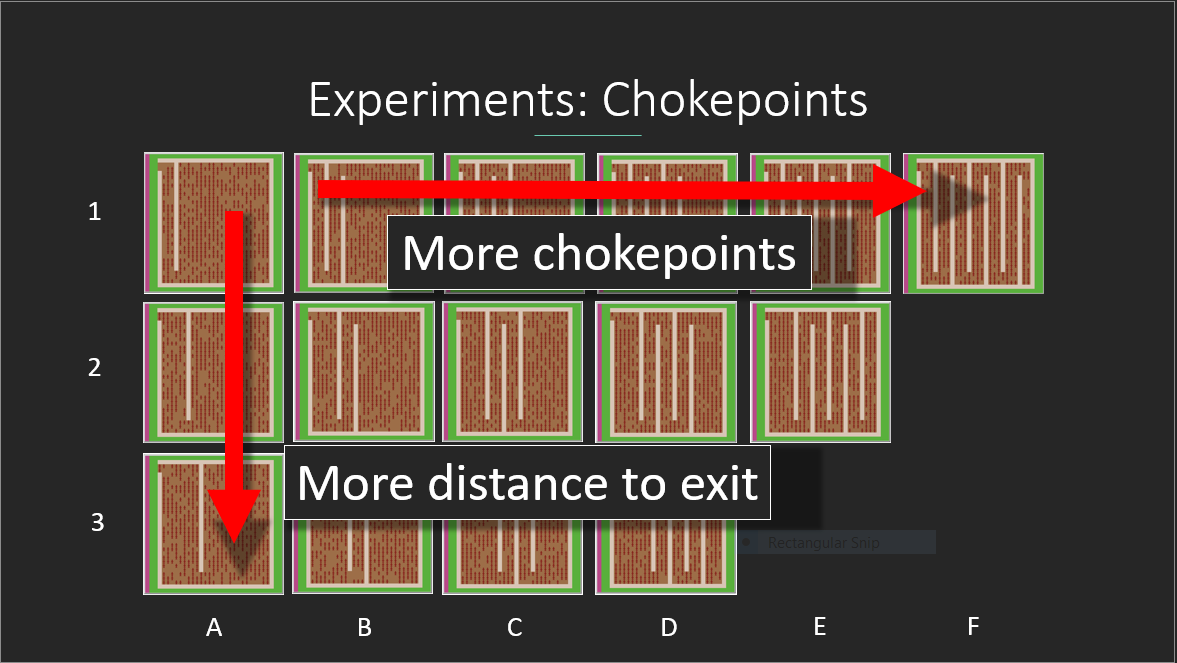
\includegraphics[width=\linewidth]{./figures/chokepoints_summary.png}
%  \caption{Chokepoint Overview}
%\end{figure}
%\begin{figure}
%  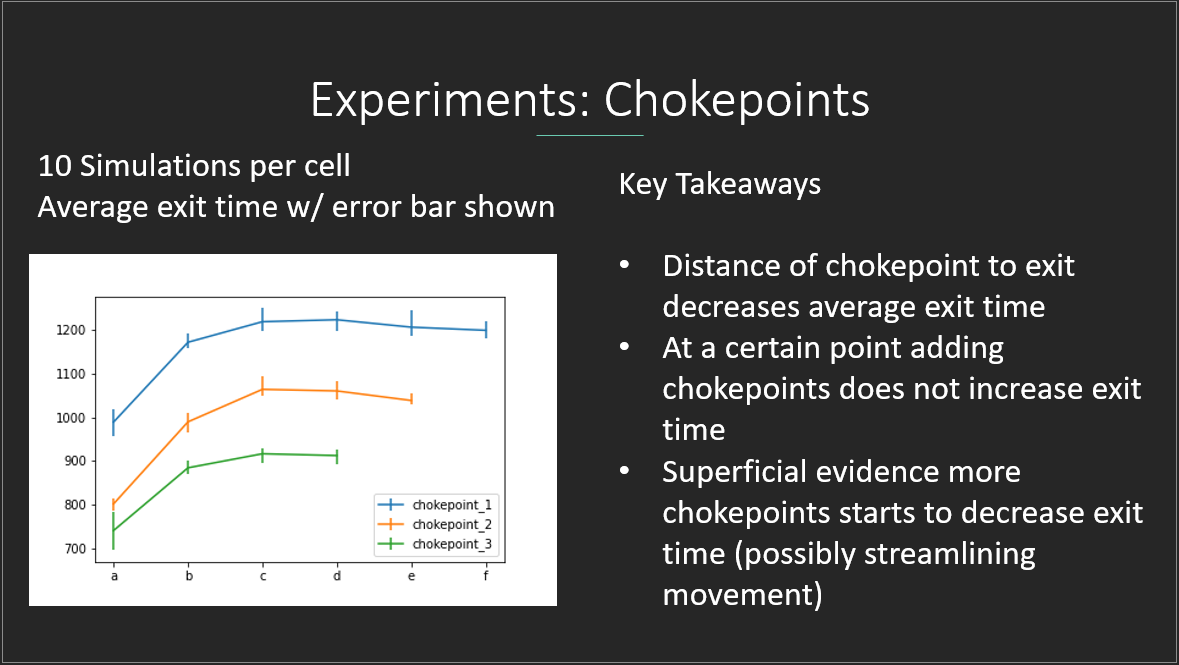
\includegraphics[width=\linewidth]{./figures/chokepoints_chart.png}
%  \caption{Chokepoint Results}
%\end{figure}
%\begin{figure}
%  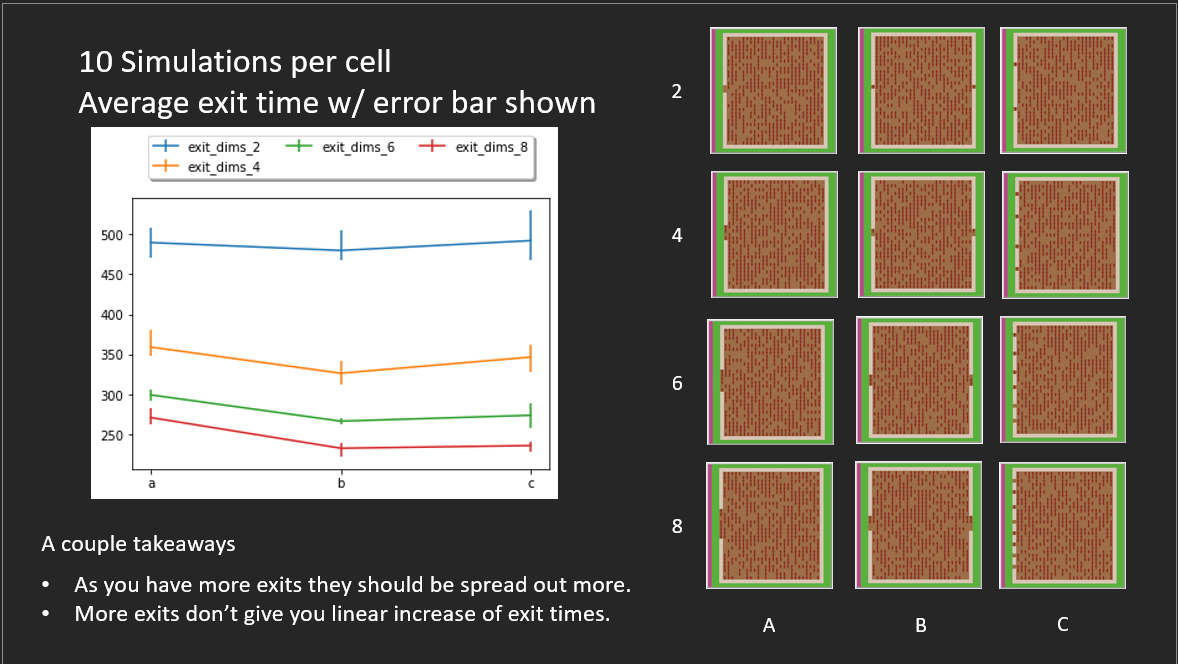
\includegraphics[width=\linewidth]{./figures/exit_dims_summary.png}
%  \caption{Exit Dimensions Overview/Results}
%\end{figure}
%\subsubsection{Experiments Replicating Emergent Crowd Behaviors}
%- mainly from this paper \cite{almeidaCrowdSimulationModeling2013}  .  
%
%\begin{figure}
%  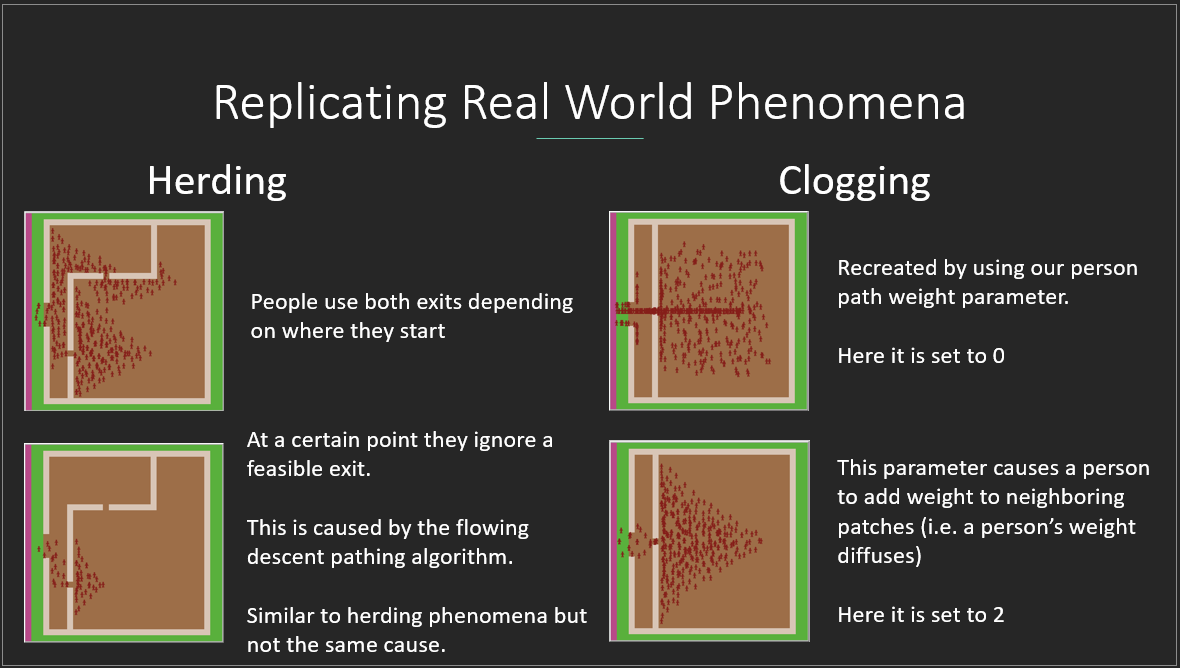
\includegraphics[width=\linewidth]{./figures/herding_clogging.png}
%  \caption{}
%\end{figure}
%
%
%if we can show that we achieve similar results even though we use a simplified pathing algorithm and abm environment i think that would be insightful


\section{Results}

The results showed that adding more length to the chokepoint pipeline did not
result in a linear increase in the exit time. Rather, the Actors resembled a
fluid dynamics problem, reaching a uniform flow and making good their escape.

More exits is better, especially if not on the same side, but there is not a
linear increase with additional exits.

\begin{figure}
  \centering
  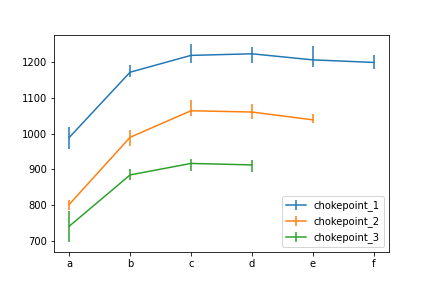
\includegraphics[width=.9\linewidth]{./figures/chokepoint_graph.png}
  \caption{Chokepoint Results}
\end{figure}
\begin{figure}
  \centering
  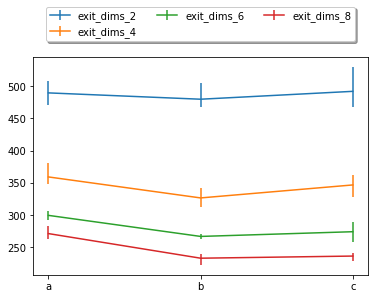
\includegraphics[width=.75\linewidth]{./figures/exit_dims_graph.png}
  \caption{Exit Dimensions Overview/Results}
\end{figure}

chokepoint1
\begin{tabular}{ r | r | r | r | r }
map & MIN  & AVG    & MAX    & VAR    \\
a &  966.4 & 1006.0 &  963.0 &  995.6 \\
b & 1155.6 & 1190.0 & 1149.0 & 1181.6 \\
c & 1207.0 & 1243.0 & 1198.0 & 1234.9 \\
d & 1217.5 & 1234.0 & 1210.0 & 1231.1 \\
e & 1202.4 & 1243.0 & 1200.0 & 1226.0 \\
f & 1183.1 & 1212.0 & 1179.0 & 1206.3 \\
\end{tabular}
\\
chokepoint2
\begin{tabular}{ r | r | r | r | r }
map & MIN  & AVG    & MAX    & VAR    \\
a &  790.8 &  833.0 &  781.0 &  819.8 \\
b &  975.7 & 1025.0 &  970.0 & 1015.7 \\
c & 1036.3 & 1071.0 & 1017.0 & 1071.5 \\
d &  103 9.3 & 10710 & 134.0 & 165.5 \\
e & 10 34. 8 & 1055.0& 102.0 & 105.2 \\  
\end{tabular}
\\
chokepoint3
\begin{tabular}{ r | r | r | r | r }
map &  MIN   & AVG   & MAX   & VAR   \\
a   &  717.6 & 758.0 & 704.0 & 751.9 \\
b   &  886.9 & 919.0 & 880.0 & 911.2 \\
c   &  905.2 & 952.0 & 900.0 & 937.3 \\
d   &  902.3 & 925.0 & 894.0 & 919.2 \\
\end{tabular}          
\\  
extdims2
\begin{tabular}{ r | r | r | r | r }
map & MIN   & AVG   & MAX   & VAR   \\
a   & 480.6 & 516.0 & 472.0 & 502.5 \\
b   & 482.9 & 522.0 & 474.0 & 510.0 \\
c   & 481.3 & 524.0 & 473.0 & 510.6 \\
\end{tabular}                          
\\
exitdims4
\begin{tabular}{ r | r | r | r | r }
map & MIN   & AVG   & MAX   & VAR   \\
a   & 348.4 & 368.0 & 342.0 & 367.3 \\
b   & 319.2 & 344.0 & 317.0 & 336.3 \\
c   & 334.3 & 365.0 & 328.0 & 358.8 \\
\end{tabular}
\\
exitdims6
\begin{tabular}{ r | r | r | r | r }
map & MIN   & AVG   & MAX   & VAR   \\
a   & 292.0 & 302.0 & 287.0 & 301.7 \\    
b   & 262.0 & 285.0 & 258.0 & 277.9 \\
c   & 265.8 & 290.0 & 265.0 & 280.3 \\
\end{tabular}
\\
exitdims8
\begin{tabular}{ r | r | r | r | r }
map &  MIN   &  AVG  & MAX   & VAR   \\
a   &  264.7 & 279.0 & 263.0 & 276.2 \\
b   &  230.4 & 243.0 & 228.0 & 240.3 \\
c   &  231.4 & 250.0 & 231.0 & 242.7 \\
\end{tabular}  

\section{Future Work}
Here we can expand on improvements we would make, additional features we could add (smoke multi-floor etc.), additional experiments, and porting to other environments

Add procedurally generated maps as mentioned in \ref{Environment}

add multilevel or 3d component

add smoke and fire spread

port to mason \footnote{https://cs.gmu.edu/~eclab/projects/mason/} or Mesa \footnote{https://mesa.readthedocs.io/en/master/tutorials/intro\_tutorial.html}

\section {Conclusion}

The simpler the layout, with more and diversified exit options, the more optimal
the evacuation results.


\bibliographystyle{plain}
\bibliography{css600}

\end{document}
